\documentclass[border=2mm]{standalone}

\usepackage{tikz}

\usetikzlibrary{positioning, chains, shapes.geometric, fit, shapes, arrows.meta, calc, backgrounds}

\begin{document}

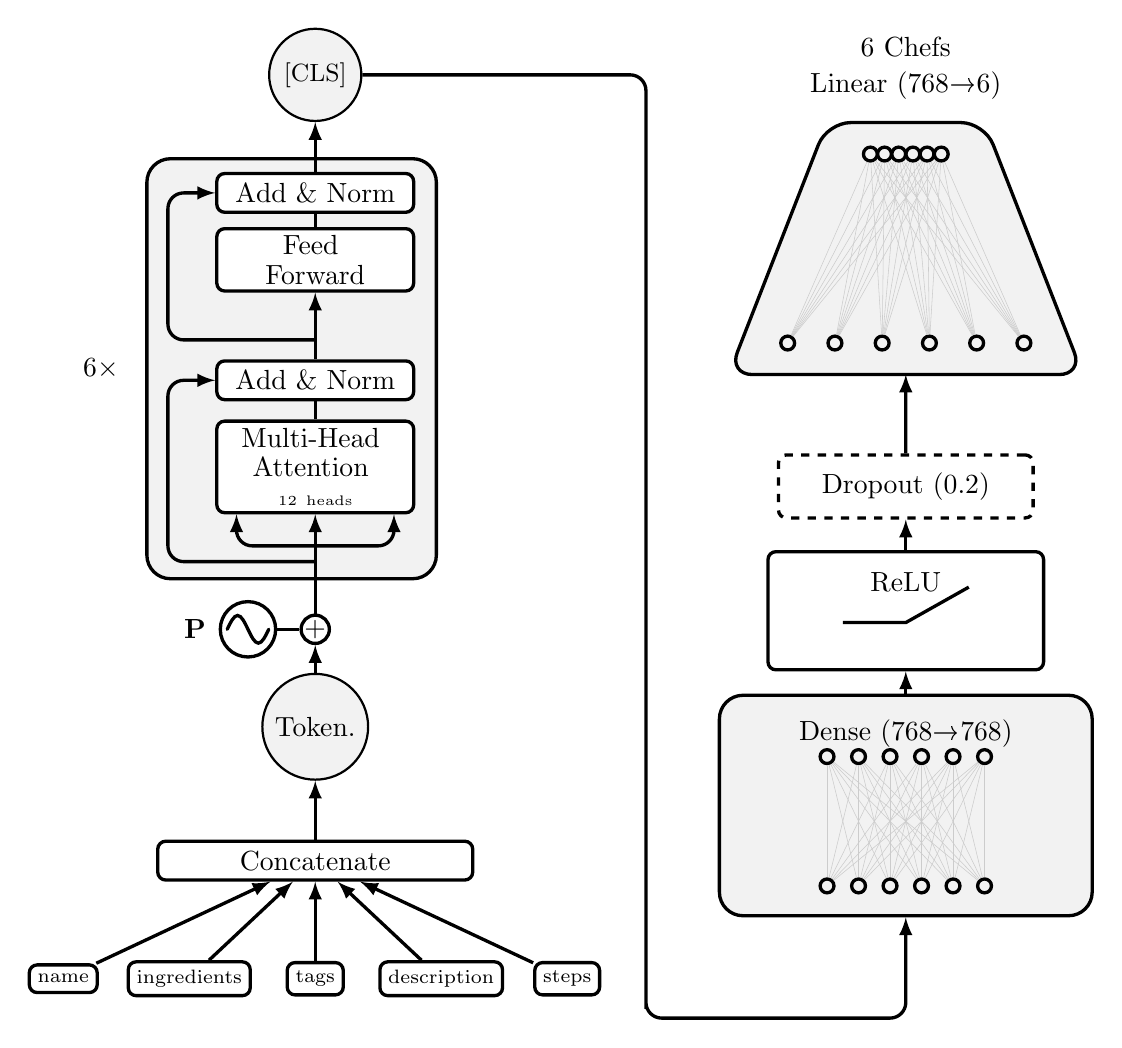
\begin{tikzpicture}[
    >=LaTeX, % Use default LaTeX arrows
    very thick,
    arrow/.style={
        -latex,
        very thick,
        rounded corners=0.2cm
    },
    block/.style={
        rectangle,
        fill=gray!10,
        rounded corners=3mm,
        draw,
        very thick
    },
    layer/.style={
        rectangle,
        fill=white!10,
        rounded corners=1mm,
        inner xsep=0em,
        inner ysep=0.25em,
        minimum height=1.4em,
        align=center,
        text width=2.5cm,
        draw,
        very thick
    },
    field/.style={
        rectangle,
        fill=white!10,
        rounded corners=1mm,
        inner sep=3pt,
        minimum height=1em,
        align=center,
        draw,
        very thick,
        font=\scriptsize
    },
    input/.style={ % Input or output node
        circle,
        minimum width=2.25em,
        draw,
        fill=gray!10,
        thick
    },
    do path picture/.style={%
        path picture={%
          \pgfpointdiff{\pgfpointanchor{path picture bounding box}{south west}}%
            {\pgfpointanchor{path picture bounding box}{north east}}%
          \pgfgetlastxy\x\y%
          \tikzset{x=\x/2,y=\y/2}%
          #1
        }
    },
    sin wave/.style={do path picture={    
        \draw [line cap=round] (-3/4,0)
        sin (-3/8,1/2) cos (0,0) sin (3/8,-1/2) cos (3/4,0);
        }
    }
]

    % Recipe fields as input (visual preprocessing)
    \node[field] (field1) at (-3.2, -4.0) {name};
    \node[field] (field2) at (-1.6, -4.0) {ingredients};
    \node[field] (field3) at (0, -4.0) {tags};
    \node[field] (field4) at (1.6, -4.0) {description};
    \node[field] (field5) at (3.2, -4.0) {steps};
    
    % Concatenation node
    \node[layer, text width=4cm] (concat) at (0, -2.5) {Concatenate};
    
    % Tokenization
    \node[input] (iemb) at (0, -0.8) {Token.};

    % Sum for positional encoding
    \node[circle, draw, minimum size=0.25em, inner sep=0pt, above=1em of iemb] (sum1) {$\mathbf{+}$};
    
    % Positional Encoding
    \node [circle, draw, sin wave, minimum size=2em, left=0.8em of sum1] (pe1) {};
    
    % Arrows from fields to concatenation
    \draw[arrow] (field1) -- (concat);
    \draw[arrow] (field2) -- (concat);
    \draw[arrow] (field3) -- (concat);
    \draw[arrow] (field4) -- (concat);
    \draw[arrow] (field5) -- (concat);
    
    % Arrow from concat to tokenization
    \draw[arrow] (concat) -- (iemb);

    % Encoder, 1st sub-layer (Multi-Head Attention)
    \node[layer] (add1) at (0,3.6) {Add \& Norm};
    \node[layer] (attn1) at (0,2.5) {Multi-Head \vspace{-0.05cm} \linebreak Attention \vspace{-0.05cm} \linebreak {\tiny 12 heads}};
    \draw[] (attn1) -- (add1);
    
    % Encoder 2nd sub-layer (Feed Forward)
    \node[layer] (add4) at (0,5.98) {Add \& Norm};
    \node[layer] (ff1) at (0,5.13) {Feed \vspace{-0.05cm} \linebreak Forward};
    \draw[] (ff1) -- (add4);

    % Encoder block background
    \coordinate (e1) at ($(attn1.south east) + (0.15,-0.7)$);
    \coordinate (e2) at ($(add4.north west) + (-0.75,0.05)$);
    \begin{scope}[on background layer]
        \node[block, fit=(e1) (e2)] (encoder) {};
    \end{scope}

    % [CLS] Token Extraction - positioned higher above encoder output
    \node[input, above=1.8em of add4, font=\small] (cls) {[CLS]};

    % Draw arrows
    \draw[arrow] (iemb) -- (sum1);
    \draw[arrow] (sum1) -- (attn1);
    \draw[] (sum1) -- (pe1);
    
    \draw[arrow] (add1) -- (ff1);
    \draw[arrow] (add4) -- (cls);
    
    % Classification head pipeline (bottom-right, flowing upward)
    % Positioned further right to extend diagram width
    
    % Dense layer with vertical neural net (768→768)
    \node[block, text width=4.5cm, minimum height=2.8cm] (dense) at (7.5, -1.8) {};
    \node[font=\normalsize, anchor=north] at ($(dense.north) + (0,-0.2)$) {Dense (768→768)};
    % Input layer (bottom) - 6 nodes representing 768 (centered)
    \foreach [count=\i from 1] \x in {-1.0,-0.6,-0.2,0.2,0.6,1.0} {
        \node[circle, draw, inner sep=1.5pt, minimum size=5pt, fill=gray!10] (din\i) at ($(dense.south) + (\x, 0.4)$) {};
    }
    % Output layer (top) - 6 nodes representing 768 (centered)
    \foreach [count=\i from 1] \x in {-1.0,-0.6,-0.2,0.2,0.6,1.0} {
        \node[circle, draw, inner sep=1.5pt, minimum size=5pt, fill=gray!10] (dout\i) at ($(dense.north) + (\x, -0.8)$) {};
    }
    % Connections - fully connected
    \foreach \i in {1,...,6}
        \foreach \j in {1,...,6}
            \draw[very thin, gray!40] (din\i) -- (dout\j);
    
    % ReLU with activation curve (smaller, white background, centered)
    \node[layer, text width=3.5cm, minimum height=1.5cm, above=0.8em of dense] (relu) {};
    \node[font=\normalsize, anchor=north] at ($(relu.north) + (0,-0.15)$) {ReLU};
    \draw[very thick] ($(relu.center)+(-0.8,-0.15)$) -- ($(relu.center)+(0,-0.15)$) -- ($(relu.center)+(0.8,0.3)$);
    
    % Dropout with dashed border (smaller, minimal design)
    \node[rectangle, draw, dashed, very thick, rounded corners=1mm, fill=white!10, 
          text width=3cm, minimum height=0.8cm, align=center, above=1.1em of relu] (dropout) 
          {Dropout (0.2)};
    
    % Linear classifier as TRAPEZOID/FUNNEL (768→6) - custom shape!
    % Draw trapezoid shape manually instead of using block style
    \coordinate (funnel_bl) at ($(dropout.north) + (-2.25, 1.0)$);  % bottom-left
    \coordinate (funnel_br) at ($(dropout.north) + (2.25, 1.0)$);   % bottom-right
    \coordinate (funnel_tl) at ($(dropout.north) + (-1.0, 4.2)$);   % top-left
    \coordinate (funnel_tr) at ($(dropout.north) + (1.0, 4.2)$);    % top-right
    
    \draw[very thick, rounded corners=3mm, fill=gray!10] 
        (funnel_bl) -- (funnel_br) -- (funnel_tr) -- (funnel_tl) -- cycle;
    
    \node[font=\normalsize, anchor=south] at ($(funnel_tl)!0.5!(funnel_tr) + (0, 0.15)$) {Linear (768→6)};
    
    % Input layer (bottom) - 6 nodes spread WIDE (representing 768)
    \foreach [count=\i from 1] \x in {-1.5,-0.9,-0.3,0.3,0.9,1.5} {
        \node[circle, draw, inner sep=1.5pt, minimum size=5pt, fill=gray!10] (lin\i) at ($(funnel_bl)!0.5!(funnel_br) + (\x, 0.4)$) {};
    }
    % Output layer (top) - 6 nodes NARROW (representing 6 chefs)
    \foreach [count=\i from 1] \x in {-0.45,-0.27,-0.09,0.09,0.27,0.45} {
        \node[circle, draw, inner sep=1.5pt, minimum size=5pt, fill=gray!10] (lout\i) at ($(funnel_tl)!0.5!(funnel_tr) + (\x, -0.4)$) {};
    }
    % Funnel connections - all inputs connect to all outputs, creating funnel effect
    \foreach \i in {1,...,6}
        \foreach \j in {1,...,6}
            \draw[very thin, gray!40] (lin\i) -- (lout\j);
    
    % Store classifier position for later arrow routing
    \coordinate (classifier) at ($(funnel_bl)!0.5!(funnel_tr)$);
    
    % 6 Chefs label above the funnel (moved higher to avoid overlap)
    \node[font=\normalsize, anchor=south] at ($(funnel_tl)!0.5!(funnel_tr) + (0, 0.7)$) {6 Chefs};
    
    % Route arrow from [CLS] to classification head (keep original working coordinates)
    \coordinate (corner1) at (4.2, 6);
    \coordinate (corner2) at (4.2, -4.5);
    \draw[arrow] (cls.east) -| (corner1) |- (corner2) -| (dense.south);
    
    % Classification pipeline arrows
    \draw[arrow] (dense) -- (relu);
    \draw[arrow] (relu) -- (dropout);
    \draw[arrow] (dropout.north) -- ($(funnel_bl)!0.5!(funnel_br)$);

    % Residual connections
    \draw[arrow] (ff1.south)++(0, -0.6) -| ($(add4.west) + (-0.6,-0.5)$) |- (add4.west);
    \draw[arrow] (attn1.south)++(0, -0.6) -| ($(add1.west) + (-0.6,-0.5)$) |- (add1.west);

    % Self-attention arrows (Q, K, V from same source)
    \draw[arrow] (attn1.south)++(0, -0.4) -| ($(attn1.south) + (-1,0)$);
    \draw[arrow] (attn1.south)++(0, -0.4) -| ($(attn1.south) + (1,0)$);

    % Labels
    \node[] at ($(pe1.west) + (-0.3,0)$) {$\mathbf{P}$};
    \node[anchor=east] at ($(encoder.west) + (-0.2,0)$) {$6\times$};

\end{tikzpicture}

\end{document}
